\chapter{第四期}

\section{2019年11月4日 星期一 晴}

余蕙琳

秋天比四季更富有果实累累的景象,我们家也是。瞧,冰箱里有着绿绿的柠檬,像个绿色的皮球,圆圆的,仔细一闻,清香四溢!再看看储物柜里的雪梨和苹果,它们真是天生绝配,一个白一个红,吃起来脆脆的,甜甜的,在储物柜的旁边,放着外公种的柿子和橘子。你看,那一个个柿子大得出奇,有一个手掌那么大,而且红得像一个个灯笼,橘子黄黄的,有些橘子皮上还布满星星点点的绿色,像给橘子涂了层眼影,和橘子一起放的还有石榴,这一个个石榴里有不少宝宝,肯定有点100多个,要是人一个有那么多的宝宝,岂不是要买20多套房子,那哪卖得起呀!现在这个是个球,圆圆的,黄黄的,大大的,它就是红柚,我家的水果能算个迷你果园。

\section{2019年11月6日 星期三 晴}

杨若君

今天晚上,我和爸爸在讨论《蝙蝠和雷达》这篇课文,针对课文来提出问题。经过讨论我们发现了很多有趣的问题。例如,如果飞机飞得很快,等无线电波反射回来的时候,飞机已经飞到了另外一个位置,那么该如何准确判断出障碍物的位置呢?如果飞机跟无线电波飞得一样快,那么被障碍物反射的无线电波岂不是永远追不上飞机,这种情况会发生吗?

看来要解决实际的问题,还真不容易啊!

\section{2019年11月6日 星期三 晴}

姚琪

我作业做完,书包理好后就上床睡觉了。躺在床上,我十分兴奋,怎么也睡不着,于是唱起歌来:“噢,妈妈,噢……”呀!“噢”这声还没唱完,我就从床上蹦起来了,原来是我的数学作业做到一半,就被妈妈催着上床了,我赶紧起来做作业。“哎!以后可不能再这么马虎了!”我小声嘟哝着。

\section{2019年11月6日 星期三 晴}

陈思涵

今天,我又去钢琴课了,面对老师严肃的表情,我心里有些忐忑不安,因为,我没练几次琴啊!我端坐在钢琴前,双手放在琴键上,十根手指灵活地在黑白琴键上欢快的跳跃着,弹奏出优美悦耳的音乐。那音乐时而雄壮,好似一首铿锵有力的进行曲;时而柔美,一首《梦中的婚礼》流入你的耳朵;时而欢快,四小天鹅又开始跳起了舞蹈;时而悲伤,仿佛看见有人在哭泣着…… 听着钢琴曲,我感觉自己也进入了当时的场景,身体开始摇摆起来…… 如果能每天听着歌写作业,再加上一块小蛋糕,那可能是世界上最浪漫的做作业方式吧!

\section{2019年11月7日 星期四 小雨}

徐诚磊

上周末发生了一件让人啼笑皆非的事。我和弟弟在玩沙,姐姐突然气冲冲的走了过来:“我的饮料是不是你喝完了?”弟弟呆萌地点了点头。“那你给瓶子里灌了什么?”姐姐的声音提高了一个分贝。“\,”自来水呀!”弟弟漫不经心地答道。姐姐拔高声音斥责道:“果然是你偷喝了我的饮料,还在里面灌了自来水又悄悄放回了原位,还害我喝了一口……”说着说着,姐姐自己被气笑出了声。大家都惊叹于弟弟的小骗局。最后姐姐因为他的诚实而放了他一马,并警告他以后再也不准这样了。

\section{2019年11月11日 星期一 晴}

余蕙琳

冷空气来临了,大街上有许许多多的变化。瞧,路旁的树枝干上涂上了白色,人们穿上了厚厚的衣服,可爱的宠物狗狗、猫猫穿上了各种各样的衣服,有“睡觉”习惯的动物们也有自己的准备的。告诉你们一个小秘密,我的衣柜里也有变化。妈妈把我的夏装换成了秋装,毛线衣、绒裤,堆满抽屉,看得我眼花缭乱。你的身边有什么变化呢?

\section{2019年11月12日 星期二 小雨}

施迪文

上周日晚上,我和马晨轩、李卓涵、孔俞橙练完球一起回家。刚出球场,只见孔俞橙朝我们晃了晃自己手中的橘子皮,猫着腰,把橘子皮放进了李卓涵的帽子里。李卓涵感到有一点不对劲,一低头,帽子里的橘子皮全掉了出来。我们哈哈大笑。

\section{2019年11月13日 星期三 小雨转阴}

陈思涵

今天,又是一个振奋人心的日子,因为,我们班今天考试!然而,向来考试又快又好的我,今天出了一些小差错,我的作文没写完!收卷时,我心里忐忑不安,好像被一根绳子吊着一样。我脑海里浮现出了画面:妈妈拿着试卷,试卷上大大的红艳艳的问号,吸引了妈妈的眼球,接着,一阵批评声传入耳窝…… 我大大的吸气,试着让自己转移注意力,但是,那个画面始终在我脑海中反复播放…… 在千钧一发之际,老师的一句:“没写完的,补上”让我长舒了一口气,心中的一块石头终于落了地。

哎,看来我还得加速写字速度!

\section{2019年11月13日 星期三}

蒋欣恬

今天发生了一件差点让我笑掉大牙的事。我刚跳完绳,只见一只猫急匆匆地跑过来,一看见我就躲在我身后,嘴里还喵喵直叫。这时一只肥老鼠跑了过来,凶神恶煞地看了看我,我哈哈大笑,这年头还有猫怕老鼠的!老鼠怪怪地冲我笑了一下,跑走了。那只猫这时从我身后跑出来,对我感激地叫了一声,然后就头也不回的跑掉了。

\section{2019年11月14日 星期三 晴}

蒋鲁弋

今天是体测日,我校举行了体测。我体前屈用尽了全力,得了满分。仰卧起坐也用尽力全力,但还是差了一点儿,没满分。肺活量鼓足力气吹,也拿了满分。当然我最骄傲的是跳绳。我们在篮球场上准备跳绳,快到我时,我手上出了好多汗,过了没一会儿,老师终止哨吹,我呼一口气,在心里默默地说:“没什么好怕的。”我准备好绳子长度,然后拉紧,这时老师吹起了哨子,我飞快地跳了起来。时间一秒一秒地过去,时间快到了,而我已经累得气喘如牛,我很想放弃,但我脑海里出现了一种声音:“加油,加油!”地叫着。我听了,用尽全身力气跳了起来,过了几秒钟,终于停了,功夫不负有心人,我终于跳了198个绳的好成绩,还被当上了单跳候选人,真是好事成双呀!看来以后都要努力做事情,才能有好结果,不能偷懒。

\section{2019年11月14日 星期三 晴}

孔俞澄

今天我在家里写作业的时候,闻到一股臭臭的味道,我仔细闻了一下会不会是妹妹在拉大便?我马上跑出房间看了一眼,不是妹妹在拉大便。心中冒出了一连串问号,我想一探究竟,就学着小狗用灵敏的鼻子闻着气味发出的方向走去。走到门口,嗯,气味就是从这里出来的。我马上走进去看,原来是爸爸在炒臭豆腐。

\section{2019年11月14日 星期四 晴}

许智涵

今天是学校体侧的日子,仰卧起坐是令我最头疼的项目。测试当时,我正憋着一肚子的气没处发泄,因为刚才的一分钟跳绳,我只跳了190个,连200都没到!仰卧起坐开始了,我闷着气,一刻不停得加速,一分钟到了,数我数的范思雯说:“行啊!52个!”啥?52个?我真怀疑我的耳朵是不是听错了,平时我只能做四十几个呀!看来,我是因为跳绳的事生了气,所以才“发疯”了吧!

\section{2019年11月14日 星期三}

徐诚磊

上周五发生了一件让我记忆深刻的事。因为我作文98分,所以老师奖我了一杯热可可,同桌对我说:“可可是巧克力融化了后的水。”一想起巧克力,我不禁口水直流三千尺。我想巧克力好吃,那么巧克力融化后的水也肯定很好吃。无奈,老师说学校里不能喝。终于放学了,我飞快地走出教室,钻进了妈妈的车。上车后,我立刻拿出杯子,拧开杯盖臭了臭:“哇,真香啊!”我喝了一大口,谁知热可可不但不甜,反而很苦,“呸呸呸,为什么这么苦呀?”我恨不得把热可可吐出来,真是“耳听为虚,口尝为实”啊!

\section{2019年11月18日 星期一 晴转小雨}

余蕙琳

“双十一”是个重要的日子,那一天人们都得把手机和银行卡刷爆,我妈就是其中一个。随之而来,有许多变化,就如小区的“喷泉池”里,瞧!“喷泉池”里堆满了包裹,简直变成了“包裹池”。据我推测,全中国加起来的包裹应该足以堆成一座“喜玛拉雅山”吧,在这个令人兴奋的日子里,那些快递员叔叔着实捏了好几把汗,他们十分辛苦,不停地搬运包裹,日夜不停地赶着。所以这个日子不仅兴奋,而且十分辛劳!在这里,我觉得应该向快递员叔叔说一声“谢谢”!

\section{2019年11月18日 星期一 晴转小雨}

赵奕麟

你有观察过烧开水的样子吗?今天我就来观察。

一开始把水都倒入烧水壶(蓝光烧水壶,是用玻璃做“身子”可看见),把水壶放上底座上,打开电源。一开始,水壶出现了小气泡,这小气泡都沉在水底,两三分钟后小气泡逐渐变大浮出水面,五六分钟过去了水完全烧开,像潮水一样,水越冲越高,这些水看上去很想逃出烧水壶啊!

\section{2019年11月18日 星期一 晴转小雨}

施迪文

上周周日,我的爸爸妈妈都很晚回家,于是我就住在孔俞橙家。我们睡觉了。我对他说:“你的钟可真亮啊!”他却说“我看不见。”我奇怪地问:“你怎么看不见了?”她回答道:“因为我有内裤。”什么?内裤戴在头上!孔俞橙可真调皮呀。

\section{2019年11月19日 星期二 晴}

蒋鲁弋

今天晚上,我的姑父来我家住。吃完饭时,我对姑父说:“我们来下盘棋吧!”姑父点了点头。于是我摆好棋,开始下了。我先来一个“当头炮”,姑父却把“马”上来了,我吃了他的“兵”,他吃了我的“炮”…… 就这样过了好久,我只剩下两个“士”,一个“将”两个“车”了,姑父高兴地说:“你要输啦!”我急得眉头皱成了一团。这时我看到了一条“必胜路”,于是我对姑父说:“你要输喽!”说完就把“车”开到了姑父的底线,姑父看到了自己的将没保护好,失望地说“我输了”。此时我尝到了胜利的甜头,还明白了一个道理:“越在危险的时候越不要慌张,只要稍微动动脑筋,还是能化险为夷的。”

\section{2019年11月19日 星期二 晴}

陈思涵

我正在看报纸,忽然,一则新闻映入了我的眼帘,吸引了我的眼球。不一会儿,两行眼泪夺目而出。是什么新闻让我感动的流泪了呢?一名快递员叔叔在午夜时分与自己的女儿视频通话,他的女儿不肯睡觉,于是,那名快递员叔叔停下电瓶车,下车给女儿跳了一段不是不是特别标准的舞。我想,人们在双十一拼命买东西,过了这一天,便躺在沙发上,看着自己的订单一点点和自己靠近,收到后,竟还有人评了差评,说送货太慢!这实在太不讲理了!要知道,一个小小的物件,饱含了快递员叔叔多少的汗水啊!不论是炎炎夏日,是寒风刺骨,还是鹅毛大雪,他们都在各处奔波。如果订单很远,他们也会坚持送货,有时,甚至打地铺睡觉,有时,还会熬夜送货。这些所有的付出,只为把订单安全送到客户的手中。真符合一句话:每个硬着骨头敢拼搏的人都有个温柔的理由。

是啊!有这么一群人,他们默默无闻地穿梭在城市的各个角落,他们是杭城一道美丽的风景线.

谢谢你们!快递员叔叔!

\section{2019年11月21日 星期四 晴}

许智涵

今天英语打卡时,我真是太烦了!第一次:“chicken”(鸡)读成“kitchen”(厨房)!第二次:“vegetable”(蔬菜)读成单数了!我不禁急得“哇哇”大叫,“轰”的一声从椅子上起来,冲进厨房,从冰箱里拿出牛奶,倒了一杯冰牛奶,猛喝一口,顿时觉得神清气爽,又回到房间,竟一下子就读好了!看来,是冰牛奶帮我那急得发热的大脑“降了降温”!

\section{2019年11月21日 星期四 晴}

夏天祺

今天詹老师给我们上了一篇选自《世说新语雅量》里的小古文,它的名字叫《王戎不取道旁李》,全文共49个字,大家不要小看这篇普普通通的小古文,这个故事可有趣了。一个七岁的小孩名字叫王戎,他在路边玩的时候,发现到路旁长着一颗李子树,上面的李子都把树枝压弯了腰,他的朋友纷纷争先恐后的去摘李子,可王戎却断定这些李子一定是苦的,因为他觉得在人来人往的大街上,要是李子很甜的话,早就被人摘光了,所以李子肯定是苦的。

我觉得王戎真是一个善于观察善于思考的人啊!我也要向他学习。

\section{2019年11月21日 星期四 晴}

孔俞澄

今天放学时我走在百合苑的沙地上,突然一个影子飞快的从我面前闪过,如同一道光,一个沙球飞过来,正中我的书包。我还没来得及躲闪又一个飞过来了。我马上转身,这些沙球都被挡了下来。之后,我不甘示弱,捏出几个沙球来防备。我轻声轻步地走了过去,一看原来是赵琪玉。我火冒三丈把所有的沙球都扔向了他。他立马给我说对不起,我也不生他的气了,我和他开开心心地回家了。

\section{2019年11月21日 星期四 晴}

徐诚磊

昨天下午因为我们公开课表现优异,所以老师奖了每对同桌一瓣柚子。我和同桌接过柚子,同桌马上说:“我们平分吧!”“好啊!”我欣然同意了,于是我们各自拿着自己的一半,津津有味地吃了起来。这是再看我的后座:张思宇和蒋鲁弋,当老师在分发时,他俩就已经急不可待了。张鲁弋一把接过柚子,眼睛直直地盯住柚子不放,说:“能不能你少一点我多一点呀?”“当然不行了!”张思宇果断拒绝。我听了忍不住笑了起来:“真是两个吃货啊!”

\section{2019年11月25日 星期一 晴}

杨若君

前几天爸爸和弟弟回老家了,我觉得家里一下子变安静了许多。每天放学回家在房间里做作业的时候什么声音也没有,只有风儿歌唱的微微响声。休息的时候可以随便玩弟弟的玩具,想怎么玩就怎么玩,没有人和我抢也没有人管我。可是这样的日子过了两天,我又有点儿想他了,因为太无聊了。可是如果他回来了,我又没自由了。

\section{2019年11月25日 星期一 晴}

蒋鲁弋

昨天去上课的时候,我坐在妈妈的车后面,妈妈正要转弯时,一辆车飞奔而来,妈妈急忙变道,刚好一辆出租车停在路边,妈妈只看左边没看右边,于是一把撞了上去。我还没看清是怎么回事,就一头撞到了妈妈的后座上。我急忙揉揉撞红的脸,发现妈妈撞了出租车。过了一会,交警来了。交警让妈妈后退一点,把两辆车分开。两车分开之后,许多部件哗哗地掉了出来,洒满了地上,水也流了很多。我对妈妈说:“妈妈,以后开车要四周多看看,不要再发生这样的事情了。”妈妈惭愧地说:“对不起宝贝们,把你们吓到了,我以后一定认真开车。”

\section{2019年11月26日 星期二 阴}

许智涵

今天,是妈妈第一次骑电动车送我上学。电动车驶出小区,转眼就到了一个红灯的路口,只见妈妈把车头一转,向右边骑车。右边又正好是一个红灯,妈妈又把车头向左一转,又骑入了通畅的道路。寒风在耳边呼啸着,周围的景物飞快得向后“跑”去。一会儿,我们就这样七拐八拐到了学校。

\section{2019年11月26日 星期二 阴}

戴瑞彤

今天跳舞前,老师问:“大家是喜欢跳舞呢?还是跳舞呢?还是更喜欢跳舞呢?”我想:老师说得不都是跳舞嘛,那肯定是喜欢跳舞啦!这时。老师对我说:“戴瑞彤,你是不是喜欢角色扮演?”我纳闷儿了,说:“老师,你为什么觉得我喜欢角色扮演呢?”老师呵呵笑了一声说:“你看看你头上就知道了。”我向上一看,两只小手摆在我的头上,还做出兔子耳朵的形状。我往后一看,原来是盛夏颖在给我扮兔子呢!盛夏颖看被我发现了,连忙逃跑。我也穷追不舍,在后面追着她,想把她也扮成兔子,可是,最后还是让她逃掉了。盛夏颖,你别以为你逃掉了,我就会放过你,明天我会报仇的。

\section{2019年11月26日 星期二 阴}

施迪文

今天放学回家的路上,我遇到了孔俞橙。于是,我们两个一边聊天一边往前走。突然,有一个人拍了我们俩一下,回头一看,是杨若君。正当她高兴的时候,一个人影出现在了她的背后,重重地拍了她一下,把她吓了一大跳。原来是李恩博。真是“螳螂捕蝉,黄雀在后”啊!

\section{2019年11月27日 星期三 晴}

蒋鲁弋

这一周,我,妈妈和爸爸都很高兴。妈妈高兴是因为外婆的田地被国家征用了,收了好几万块钱。爸爸高兴是因为他获得了保安服务证,这种证可是非常难得的,但爸爸费劲心思终于得到了这个非常难得的证。我高兴是因为在我的努力之下,虽然语文考得一般,但是数学、英语和科学都考到了95分以上,还得到了“逐浪少年”的称号,现在已经被贴在学校门口的光荣榜上了,这让我特别自豪。
这周真是好事成三呀!以后我们一家人要更加努力,获得更多的好事。

\section{2019年11月27日 星期三 阴}

姚琪

今天中午我回到教室时,看见许智涵在吃桔子,我便打算捉弄一下许智涵。来到座位上,我朝着他做了个鬼脸,许智涵塞满桔子的嘴像喷泉似的喷出了金黄色的桔子汁。我无意中忍不住打了个喷嚏——“啊啾”许智涵笑了,李恩博又模仿着我
“啊——啾”比我打的喷嚏更大声,这下,许智涵嘴里流出来的桔子汁更多了。嘿嘿,捉弄许智涵成功,耶!

\section{2019年11月27日 星期三 雨}

陈思涵

“手表”一词在我眼里有许多的含义:一是一个目标,只要我考出好成绩来,妈妈就会给我买;二是劳动的结晶,爸妈每天上班,赚钱,换来属于自己的东西…… 今天,妈妈给我买了一块嘞!我高兴极了,但我知道,这块手表,是爸爸妈妈日夜不停工作才换来的。如果没有辛苦的付出,哪有今日的微笑呢?爸妈愿意用自己的付出,换来孩子那灿烂的笑容!为了回报爸爸妈妈,我决定以后一定认真学习!

\section{2019年11月27日 星期三 阴}

蒋欣恬

今天早上我7:45就出发了。可是,老天爷还是给我制造了一场接一场的堵车。快到学校了,我们被江南大道的车给堵得水泄不通,眼看时间一点一点流走,我心乱如麻。不停地叫妈妈开快一些,我可不想再像昨天那样迟到了。终于到校,我像飞毛腿一样飞奔到教室,还好,还差三分钟就要打铃上课了。

\section{2019年11月27日 星期三 阴}

黄赫茗

今天雨下的特别大,天气也很冷,应该在10摄度以下了。放学回家的路上,雨还是一直下着,
我冷得直打颤,直到上了公交车,才感觉到一丝温暖。一到家温暖的感觉扑面而来,还是家里最舒服。

\section{2019年11月28日 星期四 晴}

夏天祺

以前考试的时候,我的阅读理解经常让我失分,最近我做了许多的练习,发现做阅读理解也是有很多技巧的,所以这次考试我的阅读理解只丢了4分,这对我来说是一个很大的进步。可是这次考试成绩却只有八十二分,因为我把作文写得太长了,考试时间到了,结尾也没写完,结果扣了十分。我很难过,可爸爸却说:“其实这也不是一个坏事,就当一个教训呗!”

\section{2019年11月28日 星期四}

徐诚磊

今天放学,妈妈对我说:“家里有一个惊喜等着你哦!”“什么啊?”我问。“保密。”妈妈说。一到家我就迫不及待地冲了进去,“哇!”我发现原来的那把旧椅子不见了,变成了一把崭新的灰色椅子,下面有轮子可以移动,还可以360度旋转,靠背上有靠垫,两边有扶手,坐上去舒服极了。但我一转身就看见那把陪伴了我五年的小椅子,正孤独地躺在客厅的一角。我非常舍不得,这时妈妈说:“这把椅子可以送给弟弟呀!”听了这话,我顿时转忧为喜,冲妈妈笑了。

\begin{figure}[htb]
    \centering
    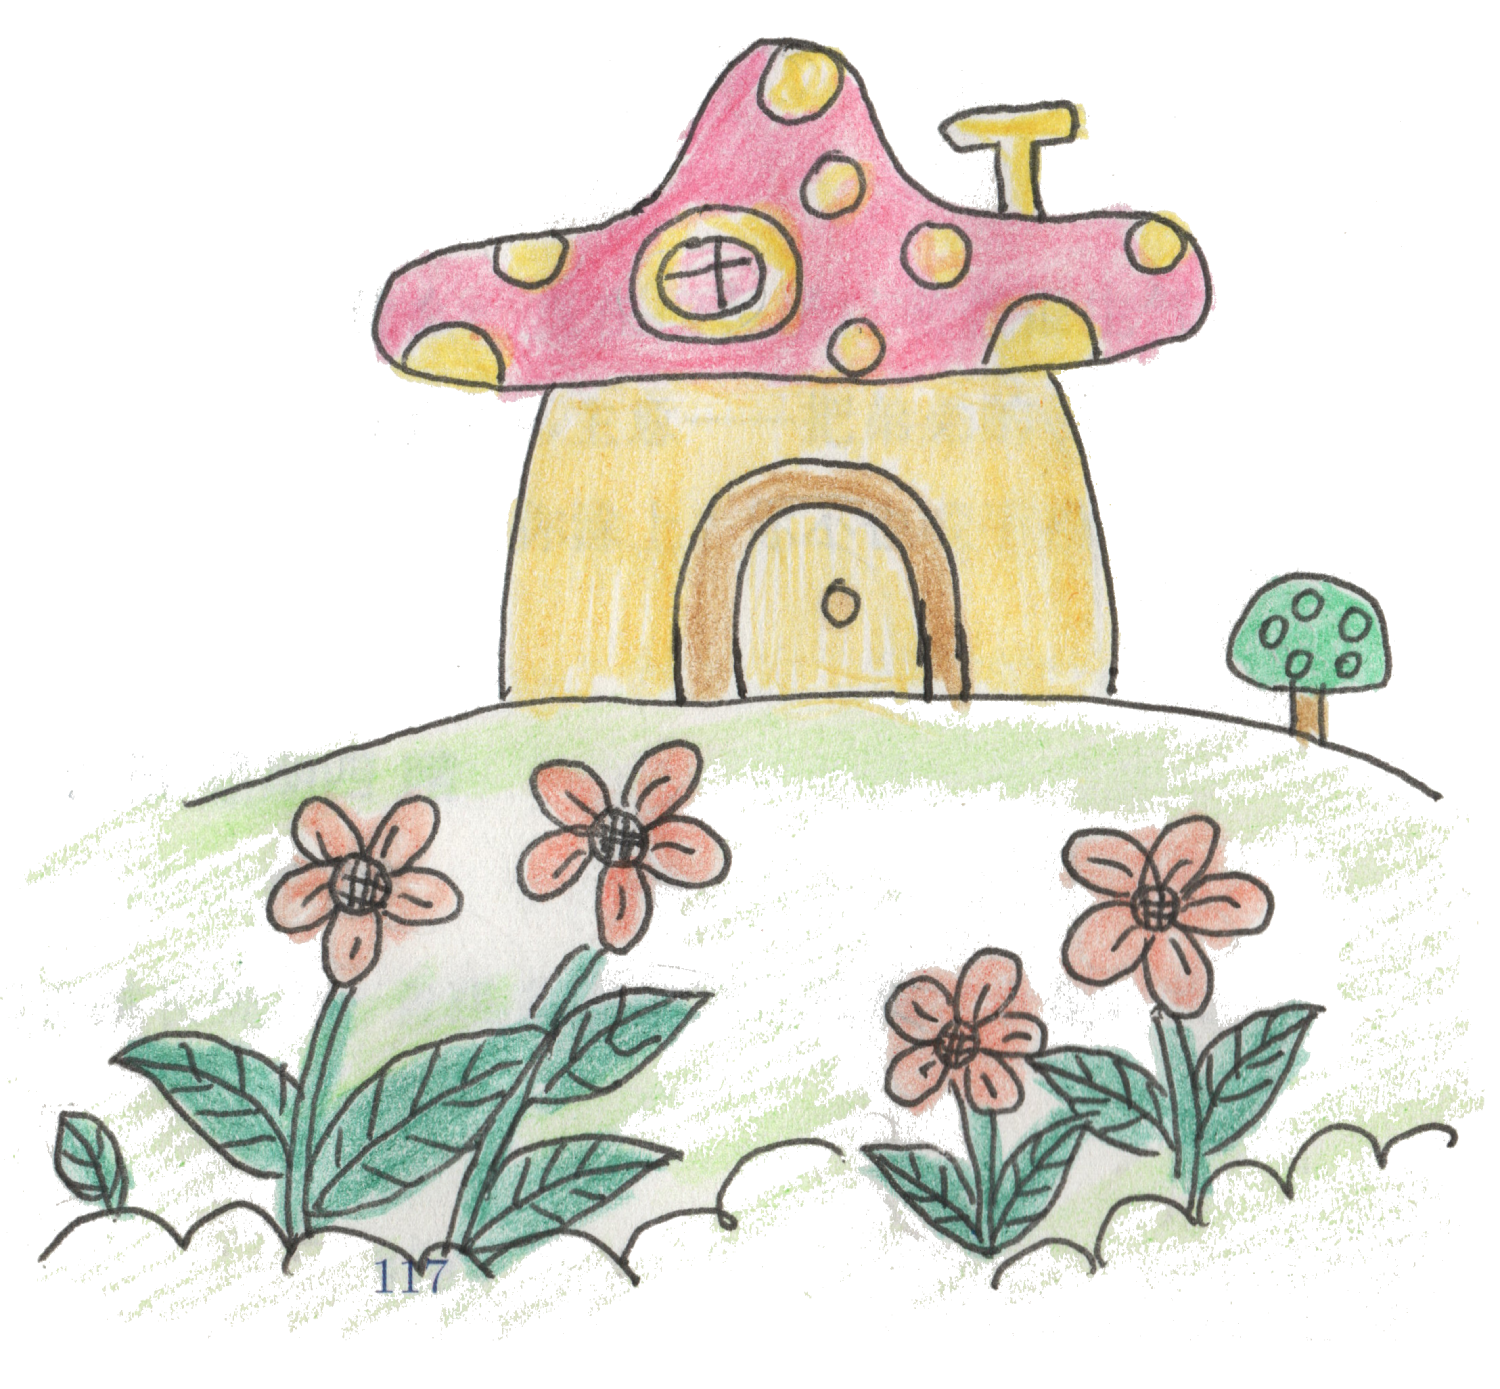
\includegraphics[width=0.8\textwidth]{figure/04.png}
\end{figure}